\documentclass[class=article, crop=false]{standalone}

\usepackage[utf8]{inputenc}
\usepackage{graphicx}
\usepackage{hyperref}
\usepackage{amsmath}
\usepackage{amssymb}
\usepackage{listings}
\usepackage[super]{nth}

\usepackage[margin=1in]{geometry}

\ifstandalone
\usepackage{color}
\usepackage{xcolor}
\usepackage{caption}
\usepackage{courier}

\lstdefinelanguage{efflang}
{
    % list of keywords
    morekeywords={
        let,
        perform,
        continue,
        val,
        effect,
        in,
        if, then, else,
        with, handle, handler,
        finally,
        match,
        exception,
        of
    },
    sensitive=false,
    morecomment=[s]{(*}{*)},
    morestring=[b]"
}

\lstdefinelanguage{scheme}
{
    % list of keywords
    morekeywords={
        define, call/cc, lambda
    },
    sensitive=false,
    morecomment=[s]{\#|}{|\#},
    morestring=[b]"
}

\lstset{
  basicstyle=\small\ttfamily, % Default font
  numberstyle=\small,          % Style of line numbers
  numbersep=5pt,              % Margin between line numbers and text
  tabsize=2,                  % Size of tabs
  extendedchars=true,
  breaklines=true,            % Lines will be wrapped
  keywordstyle=\color{red},
  frame=b,
  numbers=left,
  numberstyle=\footnotesize\color{gray},
  numbersep=10pt,
  captionpos=t,
  stringstyle=\color{purple!80!blue}\ttfamily, % Color of strings
  showspaces=false,
  showtabs=false,
  xleftmargin=17pt,
  framexleftmargin=17pt,
  framexbottommargin=4pt,
  showstringspaces=false
}

\DeclareCaptionFont{white}{\color{white}}
\DeclareCaptionFormat{listing}{\colorbox[cmyk]{0.43, 0.35, 0.35,0.01}{\parbox{\textwidth}{\hspace{15pt}#1#2#3}}}
\captionsetup[lstlisting]{format=listing,labelfont=white,textfont=white, singlelinecheck=false, margin=0pt, font={bf,footnotesize}}

\newcommand{\mylisting}[4]{%
\noindent
\begin{minipage}{\textwidth}
\lstinputlisting[
  language=#1,
  caption={#2},
  label=#3
  ]{#4}
\end{minipage}
  }

\lstset{language=efflang}
\fi

\ifstandalone
\usepackage{stmaryrd}
\usepackage{framed}

\renewcommand{\leadsto}{\rightsquigarrow}
\providecommand{\dmid}{\ \parallel \ }

\providecommand{\effFalse}{\mathbf{false}}
\providecommand{\effTrue}{\mathbf{true}}
\providecommand{\effLeft}{\mathbf{Left}\ }
\providecommand{\effRight}{\mathbf{Right\ }}
\providecommand{\effFun}{\mathbf{fun}\ }
\providecommand{\effRecFun}{\mathbf{recfun}\ }
\providecommand{\effHandler}{\mathbf{handler}\ }
\providecommand{\effVal}{\mathbf{val}\ }
\providecommand{\effWith}{\mathbf{with}\ }
\providecommand{\effHandle}{\ \mathbf{handle}\ }
\providecommand{\effIf}{\mathbf{if}\ }
\providecommand{\effThen}{\ \mathbf{then}\ }
\providecommand{\effElse}{\ \mathbf{else}\ }
\providecommand{\effAbsurd}{\mathbf{absurd}\ }
\providecommand{\effMatch}{\mathbf{match}\ }
\providecommand{\effLet}{\mathbf{let}\ }
\providecommand{\effIn}{\ \mathbf{in}\ }
\providecommand{\effRec}{\mathbf{rec}\ }
\providecommand{\effEffect}{\mathbf{effect}\ }
\providecommand{\effFinally}{\mathbf{finally}\ }
\providecommand{\effOp}{\mathtt{op}}
\providecommand{\effPerform}{\mathbf{perform}\ }
\providecommand{\tto}{\twoheadrightarrow}

\providecommand{\handlerType}{\Rightarrow}
\providecommand{\boolType}{\mathtt{bool}}
\providecommand{\unitType}{\mathtt{unit}}
\providecommand{\emptyType}{\mathtt{empty}}

\providecommand{\defEq}{\stackrel{\text{def}}{=}}

\providecommand{\cek}[1]{\langle #1 \rangle}
\providecommand{\secd}[1]{\langle #1 \rangle}
\providecommand{\shade}[1]{\langle #1 \rangle}

\providecommand{\irId}{\mathbf{Id}}
\providecommand{\irConst}{\mathbf{Const}}
\providecommand{\irBox}{\mathbf{Box}}
\providecommand{\irFun}{\mathbf{Fun}}
\providecommand{\irHandler}{\mathbf{Handler}}
\providecommand{\irVal}{\mathbf{Return}}
\providecommand{\irIf}{\mathbf{If}}
\providecommand{\irLetIn}{\mathbf{LetIn}}
\providecommand{\irLetRecIn}{\mathbf{LetRecIn}}
\providecommand{\irTopLet}{\mathbf{TopLet}}
\providecommand{\irTopLetRec}{\mathbf{TopLetRec}}
\providecommand{\irPerform}{\mathbf{Perform}}
\providecommand{\irWithHandle}{\mathbf{WithHandle}}
\providecommand{\irBinOp}{\mathbf{BinOp}}
\providecommand{\irFunApp}{\mathbf{FunApp}}
\providecommand{\irGetField}{\mathbf{GetField}}
\providecommand{\irListHead}{\mathbf{ListHead}}
\providecommand{\irListTail}{\mathbf{ListTail}}

\providecommand{\interp}[1]{\llbracket #1 \rrbracket}

\providecommand{\shUnit}{\mathbf{()}}
\providecommand{\shHalt}{\mathbf{halt}}
\providecommand{\shCast}{\mathbf{cast}}
\providecommand{\shRett}{\mathbf{ret2}}
\providecommand{\shApply}{\mathbf{apply}}
\providecommand{\shCastShadow}{\mathbf{castshadow}}
\providecommand{\shKillShadow}{\mathbf{killshadow}}
\providecommand{\shFin}{\mathbf{fin}}
\providecommand{\shThrow}{\mathbf{throw}}

\providecommand{\vmPush}{\textbf{push}}
\providecommand{\vmPop}{\textbf{pop}}
\providecommand{\vmAcc}[1]{\textbf{acc} #1}
\providecommand{\vmConst}[1]{\textbf{const} #1}
\providecommand{\vmHalt}{\textbf{halt}}
\providecommand{\vmJump}[1]{\textbf{jump }#1}
\providecommand{\vmLabel}{\textbf{label}}
\providecommand{\vmBranchIfNot}[1]{\textbf{branchifnot }#1}
\providecommand{\vmApply}{\textbf{apply}}
\providecommand{\vmRet}{\textbf{ret}}
\providecommand{\vmRett}{\textbf{ret2}}
\providecommand{\vmMakeBox}[2]{\textbf{makebox }#1, #2}
\providecommand{\vmGetField}[1]{\textbf{getfield }#1}
\providecommand{\vmListHead}{\textbf{listhead}}
\providecommand{\vmListTail}{\textbf{listtail}}
\providecommand{\vmMakeClosure}[2]{\textbf{makeclosure }#1, #2}
\providecommand{\vmMakeHlosure}[4]{\textbf{makehlosure }#1, #2, #3, #4}
\providecommand{\vmThrow}{\textbf{throw}}
\providecommand{\vmFin}{\textbf{fin}}
\providecommand{\vmCastShadow}{\textbf{castshadow}}
\providecommand{\vmKillShadow}{\textbf{killshadow}}

\providecommand{\hlosure}{\mathcal{H}}
\providecommand{\konts}{\mathcal{C}}

\newenvironment{myfigure}[4][0.75]{
    \def\mywidth{#1}
    \def\mycaption{#3}
    \def\mylabel{#4}
    \definecolor{shadecolor}{rgb}{0.95,0.95,0.95}

    \begin{figure}[#2]
    \centering
    \begin{minipage}{\mywidth\textwidth}
    \begin{shaded*}
}{
    \caption{\mycaption}
    \label{\mylabel}
    \end{shaded*}
    \end{minipage}
    \end{figure}
}
\fi

\begin{document}

This chapter is concerned with comparing the performance of my CEK interpreter
and my SHADE VM with existing solutions implementing algebraic effect handlers.
The comparison is split into two parts: to evaluate the performance of the
CEK interpreter I compare against the Eff interpreter and against the interpreter
of Multicore OCaml. The SHADE virtual machine is compared to Multicore OCaml's
byte code interpreter.

At the end of this chapter a proof of concept web server is described. This is
more of a qualitative evaluation and is supposed to show what can be done 
with effect handlers in the real-world.

\paragraph{Evaluation strategy and technical details.}

I will run multiple benchmarks each of which uses effect handlers in a different
way. Each benchmark is run 10 times and on the plots the arithmetic average of
the execution times is reported (the standard deviation is displayed as error
bars). Data was collected using GNU's \verb|time| command. During the measurements
my laptop was connected to the power supply and I tried to minimise noise in the measurements
by not running any other process (apart from a terminal) and turning off
unnecessary functionalities like WiFi, Ethernet, Bluetooth, etc.

All benchmarks are executed on a Lenovo Thinkpad X1 \nth{6} gen. with an Intel
Core i7-8565U CPU, 16GB of RAM using a single thread. The operating system in
use was a 64bit Ubuntu 18.04.4 LTS, Linux kernel version \verb|5.3.0-46-generic|.

Eff was compiled from its official GitHub repository at the time where the top
commit had SHA1 \verb|796900d|.
\footnote{The official repository is
\url{https://github.com/matijapretnar/eff/} at the time of writing.}
The version of Multicore OCaml used in the benchmarks was obtained by OPAM, the
identifier of the OPAM switch was \verb|4.06.1+multicore|.

\section{Exceptions}

The exception benchmark raises and catches exception-like effects (the
continuation is never resumed). I must add that in the OCaml benchmark I used
effects simulating exceptions rather than \emph{actual} OCaml exceptions. Actual
OCaml exceptions are implemented very efficiently in OCaml (they are not
resumable at all).

\begin{figure}
    \centering
    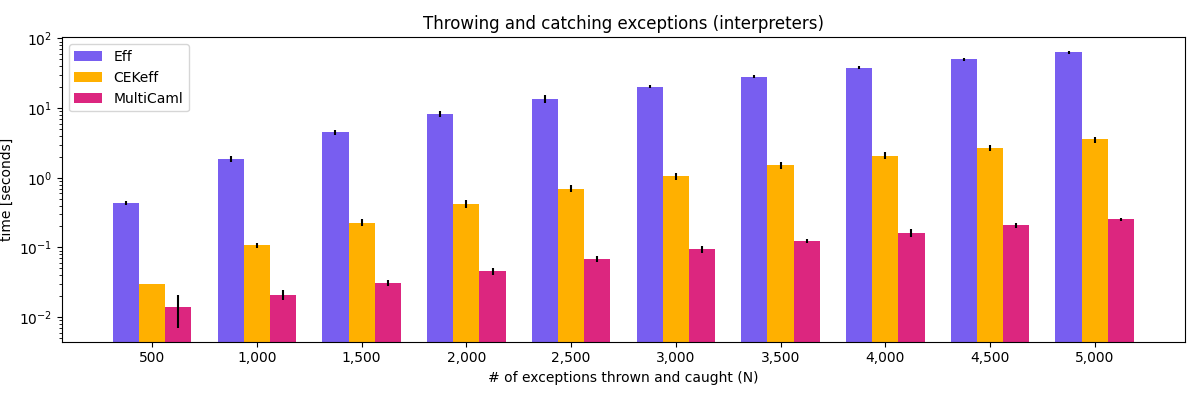
\includegraphics[width=40em]{eval_plots/interp_exception.png}
    \caption[Exception benchmark with interpreters]{The CEK interpreter performs better than Eff but worse than
    Multicore OCaml}
    \label{fig:exception-interpreters}
\end{figure}

\autoref{fig:exception-interpreters} shows that the OCaml interpreter beats
the CEK interpreter in this benchmark. However, we can see on
\autoref{fig:exception-bytecode} that the performance of SHADE VM is
comparable to Multicore OCaml's VM even though the
execution time for SHADE includes the compilation time to SHADEcode,
but the times for Multicore OCaml do not include compilation. As I did not
implement serialization for my byte code Eff programs were recompiled every time
a SHADE benchmark was run. However, this extra time is less and less significant
as we increase the number of exceptions.

\begin{figure}
    \centering
    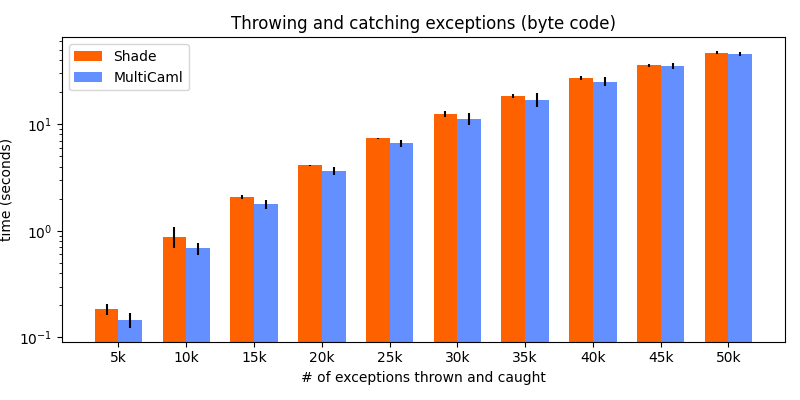
\includegraphics[width=35em]{eval_plots/comp_exception.png}
    \caption[Exception benchmark with compilers]{The peformance of SHADE is comparable to Multicore OCaml's}
    \label{fig:exception-bytecode}
\end{figure}

Note that as the byte code solutions are vastly more efficient than their
interpreter counterparts they are compared with a larger number of exceptions.
It takes around 63 seconds for the Eff interpreter to evaluate the benchmark
with 5000 exceptions, whereas this takes only 3.5 seconds for the CEK
interpreter. For SHADE VM the same takes around 200 milliseconds
(with compilation included), which is a 300-fold improvement!

The $y$-axis is logarithmic and the plots show a linear slowdown when we
increase the number of exceptions linearly. This suggests an $\mathcal{O}(N)$
time complexity for performing and catching $N$ exceptions which suggests that
my implementation does not contain bugs or inefficiencies that accumulate
as more effects are performed in a program.

\section{State and I/O}

The state benchmark implements an integer state which gets incremented every
time an \verb|Incr| effect is performed. The handler of the \verb|Incr| effect
resumes a continuation exactly once. The reason why I chose such a 
computationally cheap operation as integer addition is that I wanted to measure
the performance of performing effects and resuming continuations. As the number
of performed effects $N$ increases we can be confident that the cost of
performing effects and resuming continuations will dominate the execution time
and that we are measuring what we want.

\begin{figure}
    \centering
    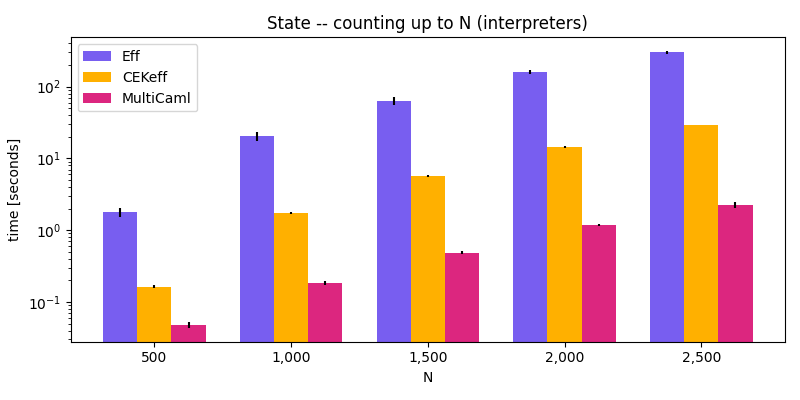
\includegraphics[width=35em]{eval_plots/interp_state.png}
    \caption[State benchmark with interpreters]{Again, the CEK interpreter performs better than Eff but worse than
    the interpreter of Multicore OCaml}
    \label{fig:state-interpreters}
\end{figure}

\begin{figure}
    \centering
    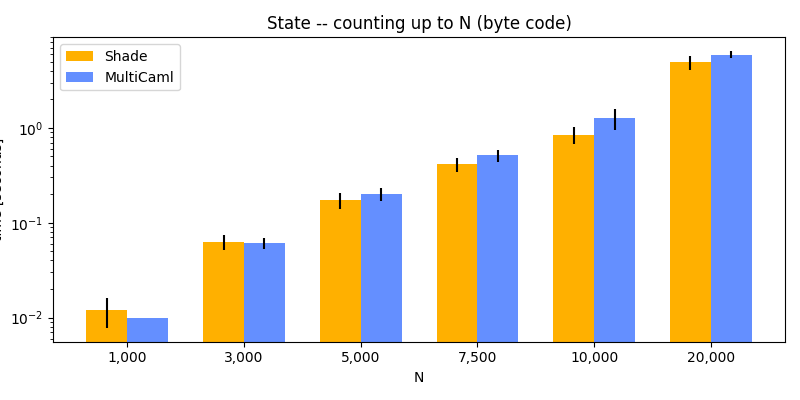
\includegraphics[width=35em]{eval_plots/comp_state.png}
    \caption[State benchmark with compilers]{SHADE VM's performance is still head-to-head with Multicore OCaml}
    \label{fig:state-bytecode}
\end{figure}

The results are displayed on \autoref{fig:state-interpreters} and
\autoref{fig:state-bytecode}. The interpretation of these results is similar to
the exception case although they reveal a \emph{very important property} of the implementation.

In the exception case the size of the dump in SHADE VM remained constant.
However, in this case the size of the dump grows
linearly with $N$. As the dump is essentially a linked list of shadows residing
in the heap it is reassuring to see that the performance does not degrade
rapidly with $N$. In fact, we see an $\mathcal{O}(N)$ slowdown again, which is
what one would expect from any efficient implementation (but we would not want a
solution where the cost of performing an effect or resuming a continuation grows
like $\mathcal{O}(N^2)$ for instance).

\section{Non-determinism -- Solving the N-queens problem}

The $N$-queens
\footnote{The N-queens problem is concerned with finding the positions of $N$
queens on an $N \times N$ chessboard such that no two queens attack each other.}
benchmark is a backtracking program which resumes continuations more than once.
Here I do not compare against the CEK interpreter for the bigger benchmarks
because due to its naïve implementation it slows down significantly after
$N > 14$. 

\begin{figure}
    \centering
    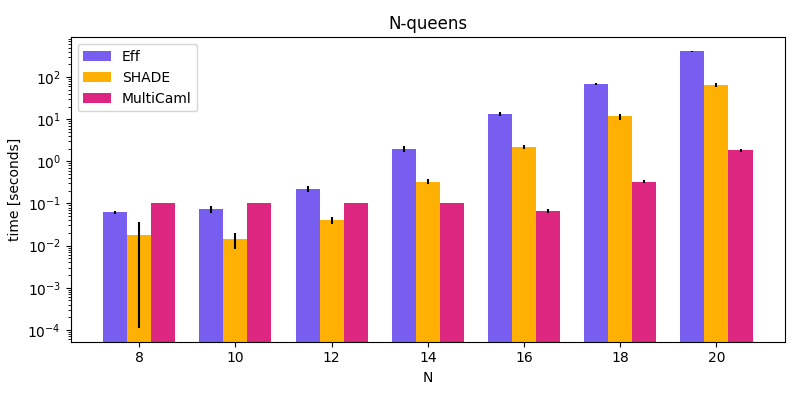
\includegraphics[width=35em]{eval_plots/comp_queens.png}
    \caption[N-queens benchmark]{SHADE VM loses against Multicore OCaml here but is still more
    performant than the Eff interpreter}
    \label{fig:n-queens}
\end{figure}

The performance of SHADE VM remains acceptable, although worse than the VM of
Multicore OCaml as \autoref{fig:n-queens} shows.

The reason why Multicore OCaml performs so much better than SHADE VM was
already mentioned briefly in the Implementation chapter. Multicore OCaml implements
\emph{one-shot continuations} and relies on the user to specify when a continuation
should be cloned.

\mylisting{caml}
{[Explicit continuation cloning in Multicore OCaml]Cloning continuations must be done explicitly in Multicore OCaml}
{lst:multicaml-cloning}
{../code_examples/multicaml_cloning.ml}

\begin{figure}
    \centering
    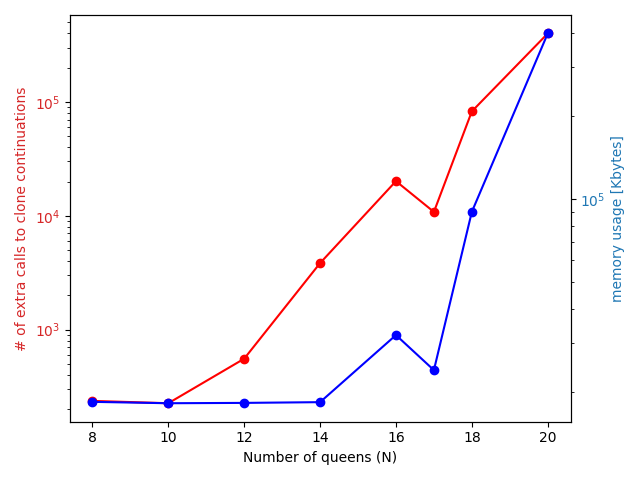
\includegraphics[width=35em]{eval_plots/extra_cloning.png}
    \caption[Correlation between extra cloning and memory usage]{Investigating the effect of cloning on performance and memory usage}
    \label{fig:extra-copying}
\end{figure}

\autoref{fig:extra-copying} reveals the extent to which this extra cloning
affects SHADE VM's performance. I added a counter to my runtime system just for
this benchmark to measure how many times continuations were cloned (the original
benchmark did not have such a counter as I did not want performance monitoring
to interfere with my results, i.e., the two metrics were measured in separate
runs). We see that there is a good correlation between the number of extra
clone calls and the memory used in the program. It is also possible to determine
the average size of a continuation from the raw data. It turns out that the typical
size of continuations is between 1 and 2 Kbytes (based on the bigger test cases, i.e.,
where $N$ is 16, 18 or 20).

\subsection{Vulnerability of the evaluation}

A subtlety must be pointed out here. The $N$-queens benchmark traverses a huge
search space of all $N$-queen configurations on an $N\times N$ chessboard. The
order in which we inspect the configurations \textbf{does} matter here.

If one were to repeat this experiment one would have to ensure that their
backtracking strategy is the same if they wish to compare their results to this
evaluation. I used the same strategy in all my measurements and although this is
a popular benchmark I do not compare my results with benchmarks from other papers
as the papers often do not mention what strategy they use.

An even more subtle point is that $N$ matters too. One must not fall in the pitfall
of comparing the results for cases with different sizes (\autoref{fig:extra-copying}
reveals for instance that the $N=10$ case is actually ``easier'' than the $N=8$
case) as $N$ does not represent the complexity of the problem, it is merely the
identifier of a big search space. Interestingly, the $N=8$ and $N=10$ cases are
nearly always reported in papers whereas the $N=17$ is consistently left out as
it is an obvious outlier.

\section{Concurrency -- Hello Online World!}

Cooperative multitasking can be implemented with algebraic effects and their
handlers too. We can realise \emph{green threads}\footnote{Green threads are
lightweight user space threads usually scheduled by runtime systems rather
than the operating system.} as $\unitType \to \unitType$
functions which can be \lstinline|Spawn|ed and which are capable
of \lstinline|Yield|ing control. The reader might correctly suspect that
these operations will correspond to algebraic effects with the following types:

\mylisting{efflang}
{Effects for implementing a Hello World webserver}
{label}
{../code_examples/yield_spawn.eff}

I built in two additional asynchronous effects in the runtime system of
SHADE VM: \verb|Accept| and \verb|HTTPHello|.
Both effects use non-blocking Unix system calls under the hood.
\verb|Accept| can accept an incoming network connection on port 8080 and returns
the new port number that can be used for further communication with a client.
The \verb|HTTPHello| effect takes a port number and sends a ``Hello World!''
HTTP message using an already established connection.

Now we can implement two types of green threads: the function
\lstinline|start_server| implements the main thread of the web server: it
accepts connections on the port 8080. If there is a new connection then a new
green thread is spawned for that connection, otherwise control is given to other
threads.

\mylisting{efflang}
{Main green thread of the web server}
{label}
{../code_examples/start_server.eff}

The \lstinline{say_hello} function takes a port number and
\emph{returns a green thread}: a $\unitType \to \unitType$ function that will
send the ``Hello World'' message on the port given but only if the underlying
socket is ready. If this is not the case it yields control and will retry later.

\mylisting{efflang}
{Green thread handling a connection}
{label}
{../code_examples/say_hello.eff}

As effect handlers can simulate state it is possible to implement thread
scheduling with handlers too. The web server thus can be started with something
like \lstinline{with thread_scheduler handle start_server ()}.

Based on the work of Dolan et al. \autoref{dolan2017concurrent} I claimed in
the Introduction that effect handlers give flexibility to programmers to
implement their own concurrency models which suits their application the most
while they reduce the complexity of runtime systems. This is a justification of
that claim (it is actually a simplified experiment from their paper). We see
that \lstinline|thread_scheduler| could implement any kind of scheduling policy by
handling the \lstinline|Yield| and \lstinline|Spawn| effects appropriately. The fact that
one can implement a toy webserver using one's own runtime system written from
scratch in less than a year justifies the second claim (the cited paper is a
result of the collaboration of 6 people).

I load tested this web server with the \lstinline|wrk2| load testing tool
\cite{wrk2-website} using 4 threads and gradually increasing the number of
connections until the p90 time fell below the 5s threshold (this happened at
around 100 connections as the red numbers indicate this on
\autoref{fig:hello-online-world}.

\begin{figure}
    \centering
    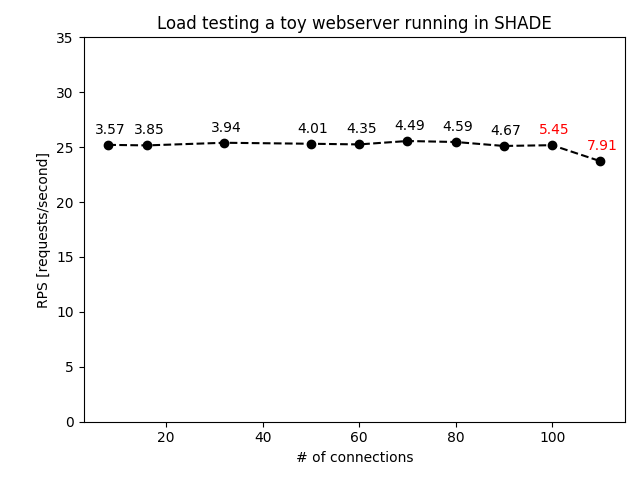
\includegraphics[width=30em]{eval_plots/webserver.png}
    \caption[Load testing a toy webserver]{Although the performance of the webserver is not at all impressive,
    it is my own runtime system that implements it and it can still handle 100
    connections with a p90 time of 5 seconds with a throughput of 25 requests
    per second.}
    \label{fig:hello-online-world}
\end{figure}

\section{Summary}
The following sums up this chapter and reports its findings.
\begin{itemize}
\item The performance of the syntax-level CEK interpreter and the SHADE VM was
compared to Eff and Multicore OCaml.
\item My CEK interpreter was 20x quicker on the exception benchmarks and 10x
quicker on the state benchmarks than the Eff interpreter. However, it was also
15x slower on both the exception and state benchmarks than the OCaml interpreter.
\item My SHADE VM was consistently quicker than all the interpreters and
performed well on the exception (SHADE is 2\% slower) and state benchmarks
(SHADE is 17\% quicker) against the VM of Multicore OCaml. However,
it remained around 35x slower than the VM of Multicore OCaml on the $N$-queens
benchmark.
\item The reason for this slowdown on the $N$-queens benchmark
was determined and it was found that the cause is inherent in Eff. Eff supports
multi-shot continuations, whereas Multicore OCaml only supports one-shot
continuations and therefore the copy overhead in the SHADE VM is bigger.
\item As a qualitative evaluation of SHADE a toy webserver was presented and
load tested.
\end{itemize}

\end{document}
